\documentclass[12pt]{article}
\usepackage[english]{babel}
\title{StatCrunch Competition\\ Twitch Dataset}
\author{Matthew Carson\\ University of California, Los Angeles}
\date{\today}

\usepackage{amsmath}
\usepackage{url}
\usepackage{hyperref}
\usepackage{graphicx}
\usepackage{float} % for [H] placement specifier
\usepackage{caption} % for customizing captions
\usepackage[margin=1in]{geometry} % for setting margins
\usepackage{setspace} % for adjusting line spacing
% Line spacing
\setstretch{1.25}
\usepackage[autostyle, english = american]{csquotes}
\MakeOuterQuote{"}

% Define indentation length
\newlength{\myindent}
\setlength{\myindent}{3em}

% Paragraph indentation
\setlength{\parindent}{\myindent}

%%%%%%%%%%%%%%%%%%%%%%%%%%%%%
% Begin Document
% Title Page
%%%%%%%%%%%%%%%%%%%%%%%%%%%%%
\begin{document}
\begin{titlepage}
\maketitle
\thispagestyle{empty} % Removes page number from the cover page
\end{titlepage}
% Set page numbering to roman for preliminary pages
\pagenumbering{roman}
%%%%%%%%%%%%%%%%%%%%%%%%%%%%%
% Table of Contents
%%%%%%%%%%%%%%%%%%%%%%%%%%%%%
\tableofcontents

%%%%%%%%%%%%%%%%%%%%%%%%%%%%%
% List of Tables
%%%%%%%%%%%%%%%%%%%%%%%%%%%%%
\listoftables

%%%%%%%%%%%%%%%%%%%%%%%%%%%%%
% List of Figures
%%%%%%%%%%%%%%%%%%%%%%%%%%%%%
\listoffigures
\newpage
%%%%%%%%%%%%%%%%%%%%%%%%%%%%%
% Begin body of report
%%%%%%%%%%%%%%%%%%%%%%%%%%%%%
% Set page numbering to arabic for main content
\pagenumbering{arabic}

\section{Summary Statistics}\

Since these data were not randomly sampled, it would be inappropriate to conduct inference (i.e., construct confidence intervals or conduct hypothesis tests). Because of this, it is not possible to estimate population parameters; that is, make claims or generalizations about the broader population of Twitch users. However, since these data represent the top 900 Twitch users, statistics can be calculated and relationships can be discovered about that population.

Initial calculations were made before presenting the summary statistics. Since values for \texttt{`Watch time (mins)'} were typically very large, requiring scientific notation to express, values were rescaled to \texttt{`Mean weekly watch hours’} by dividing \texttt{`Watch time (mins)'} by the product of 60 times 52 (number of weeks in a year) to make the numbers more manageable:

\begin{equation}
Mean\ weekly\ watch\ hours = \dfrac{Watch\ time\ (mins)}{60 \ast 52}
\end{equation}
\newline
Additional statistics were calculated as well:

\begin{itemize}
	\item \texttt{`Followers Prev Yr’} = \texttt{`Followers’} - \texttt{`Followers gained’}.
	\item \texttt{`Followers gained percent’} = \texttt{`Followers gained’} / \texttt{`Followers Prev Yr’}.
\end{itemize}

Because all distributions are heavily right skewed (skewness $\geq$ 2.6), medians, represented with Greek letter eta ($\eta$), are reported instead of means (all values are from Table \ref{table:summary_stats}). The majority of the top nine hundred accounts stream content at least 30 hours per week ($\eta \approx$ 34.23) and are watched more than 90 thousand hours per week $(\eta \approx$ 91,422). 
%%%%%%%%%%%%%%%%%%%%%%%%%%%%%
% Table: Summary Statistics
%%%%%%%%%%%%%%%%%%%%%%%%%%%%%
\begin{table}[b]
  \centering
  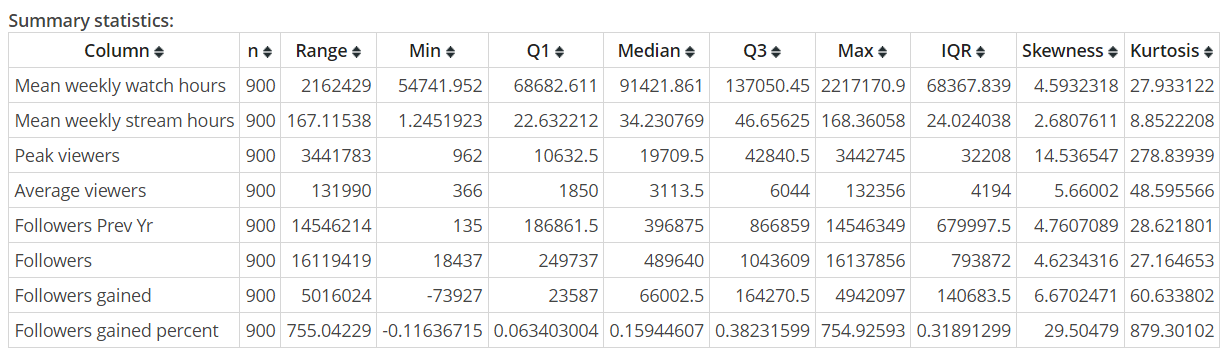
\includegraphics[width=\linewidth]{../StatCrunch_Results/table}
  \captionsetup{justification=centering, singlelinecheck=false, margin=2cm}
  \caption[Summary Statistics]{Summary Statistics.}
  \label{table:summary_stats}
\end{table}
\noindent
Most accounts gained a substantial number of followers from the previous year ($\eta \approx$ 66,003), which represents a median increase of approximately 16 percent. Because of the heavy skewness of the distributions, easy-to-interpret visualizations were difficult to make (Fig. \ref{fig:histogram_matrix}).

\section{Correlation}

To assess the relationships between numeric variables, Spearman’s correlation coefficients were calculated (Fig. \ref{fig:spearman_correlogram}). Because of the non-linearity of the relationships (Fig. \ref{fig:stream_scatter_matrix}), typical Pearson’s R correlation coefficients would be inappropriate. Spearman’s correlation coefficients are preferred for assessing the strength of non-linear relationships.
%%%%%%%%%%%%%%
% Figure: Spearman Correlogram
%%%%%%%%%%%%%%
\begin{figure}[H]
  \centering
  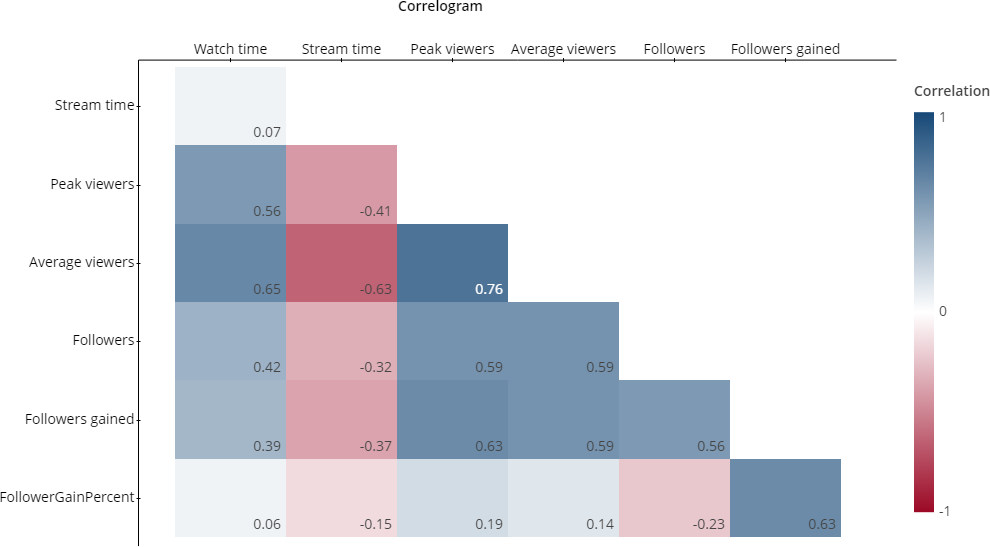
\includegraphics[width=\linewidth, height=0.4\textheight]{../StatCrunch_Results/spearman_correlogram}
  \captionsetup{justification=centering, singlelinecheck=false, margin=2cm}
  \caption[Spearman Correlogram]{Spearman Correlogram}
  \label{fig:spearman_correlogram}
\end{figure}

The relationships between numeric variables are surprising, especially the absence of some correlations where one would think they they would exist (Fig. \ref{fig:spearman_correlogram}). \texttt{`Stream time’} has a moderately strong negative Spearman correlation ($\rho$) with \texttt{`Average viewers’} ($\rho = -0.63$), which is counterintuitive given that one might expect more frequent streaming to result in more viewers, but that is not the case. In terms of change over time, accounts that streamed more hours did \emph{not} gain more followers; indeed, the accounts that were in the top decile of weekly stream time gained less than one-fifth of the followers that the accounts in the lowest stream time decile gained (Table \ref{table:followers_gained_stream_decile_table}; Fig. \ref{fig:followers_gained_stream_deciles}).  With respect to surprising absences of relationships, \texttt{`Stream time’} has practically no relationship with \texttt{`Watch time’} ($\rho = 0.07$; Fig. \ref{fig:spearman_correlogram}). Together, these findings suggest that a strategy of merely increasing one’s streaming time does not “pay off” in terms of the number of followers or viewers.

%%%%%%%%%%%%%%%%%%%%%%%%%%%%%
% Table: followers_gained_stream_decile_table
%%%%%%%%%%%%%%%%%%%%%%%%%%%%%
\begin{table}[!h]
  \centering
  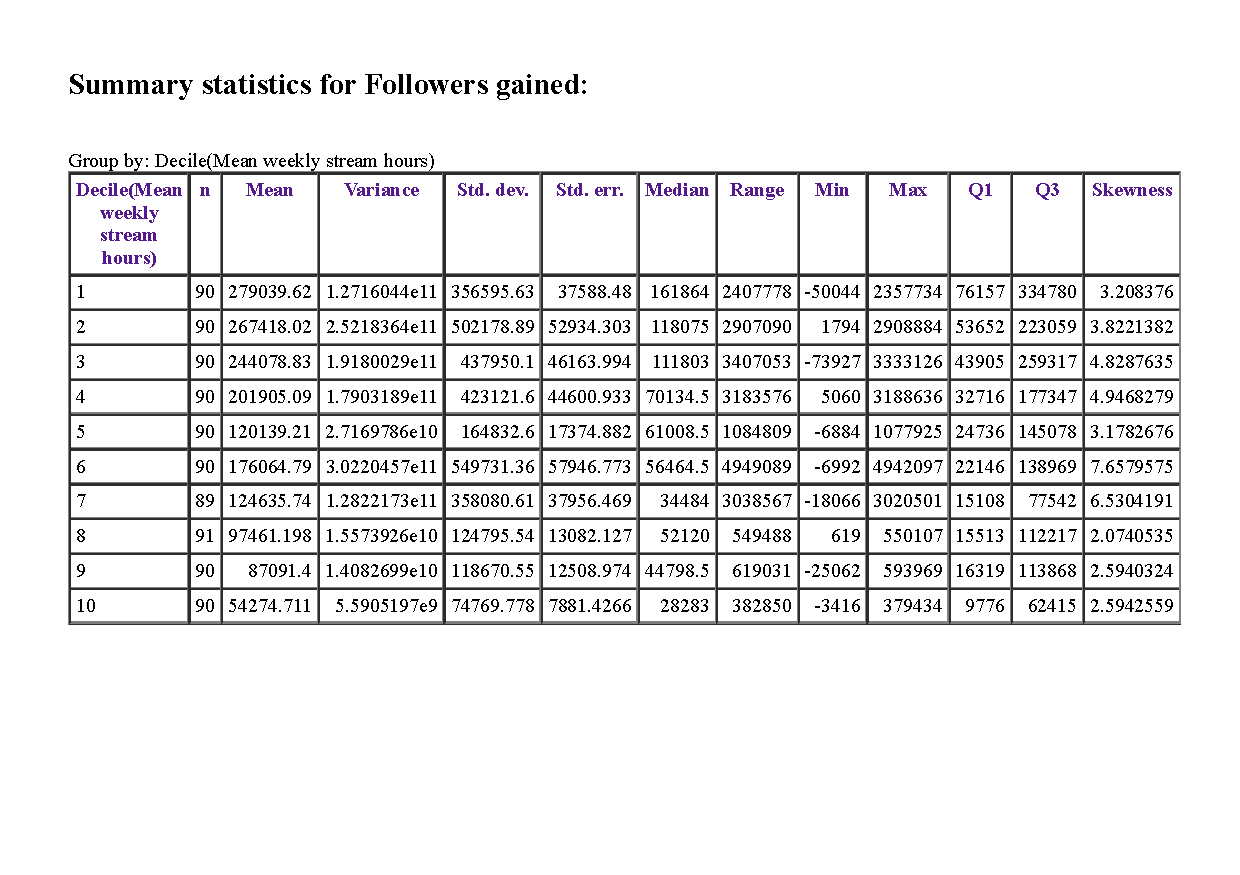
\includegraphics[width=\linewidth, height=0.25\textheight]{../StatCrunch_Results/followers_gained_stream_deciles/table}
  \captionsetup{justification=centering, singlelinecheck=false, margin=2cm}
  \caption[Followers Gained by Stream Time Deciles]{Followers Gained by Stream Time Deciles. (The lowest decile streamed the least.)}
  \label{table:followers_gained_stream_decile_table}
\end{table}


%%%%%%%%%%%%%%%%%%%%%%%%
% Figure: followers_gained_stream_deciles
%%%%%%%%%%%%%%%%%%%%%%%%
\begin{figure}[!b]
  \centering
  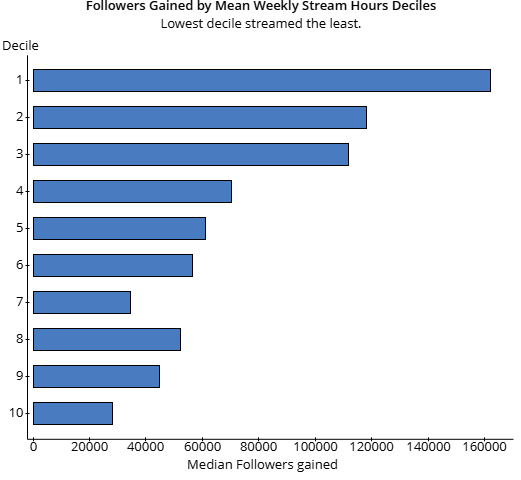
\includegraphics[width=0.8\linewidth, height=0.35\textheight]{../StatCrunch_Results/followers_gained_stream_deciles/barplot}
  \captionsetup{justification=centering, singlelinecheck=false, margin=2cm}
  \caption[Followers Gained by Stream Time Deciles]{Followers Gained by Stream Time Deciles. (The lowest decile streamed the least.)}
  \label{fig:followers_gained_stream_deciles}
\end{figure}

\section{Simple Linear Regressions}\

Because the relationships between the variables were not linear, it was difficult to fit models using simple linear regression. However, using transformations, I was able to fit some models.

\subsection{Stream Hours to Predict Average Viewers}\

A simple linear regression was run to assess the strength between \texttt{`Mean weekly stream hours’} (independent variable) and \texttt{`average viewers’} (dependent variable). Because of the non-linear relationship between the variables, the residuals were highly non-normal. A inverse (reciprocal) transformation of \texttt{`Average viewers’} was performed to correct for non-normality of the residuals. The transformation greatly improved the distribution of the residuals, making them nearly normal. The transformation could not correct for heteroskedasticity, but this is not an issues since inference is not being conducted.

\subsubsection{Model Specification}

The regression model is as follows:

\begin{equation}
\dfrac{1}{Average\ viewers_{i}} = \beta_{0} + \beta_{1} \ast Mean\ weekly\ stream\ hours_{i} 
\end{equation}
where \textit{i} is a Twitch account. \textit{`Average viewers'} is the average number of viewers that watched the respective Twitch account; and \textit{`Mean weekly stream hours'} is the number of hours that the respective Twitch account streamed over the year divided by 52.

\subsubsection{Results}

%The regression results are reported below (Table \ref{table:reciprocal_regression_table}).

%%%%%%%%%%%%%%%%%%%%%%%%%%%%%
% Table: Regression table
%%%%%%%%%%%%%%%%%%%%%%%%%%%%%
\begin{table}[!h]
  \centering
  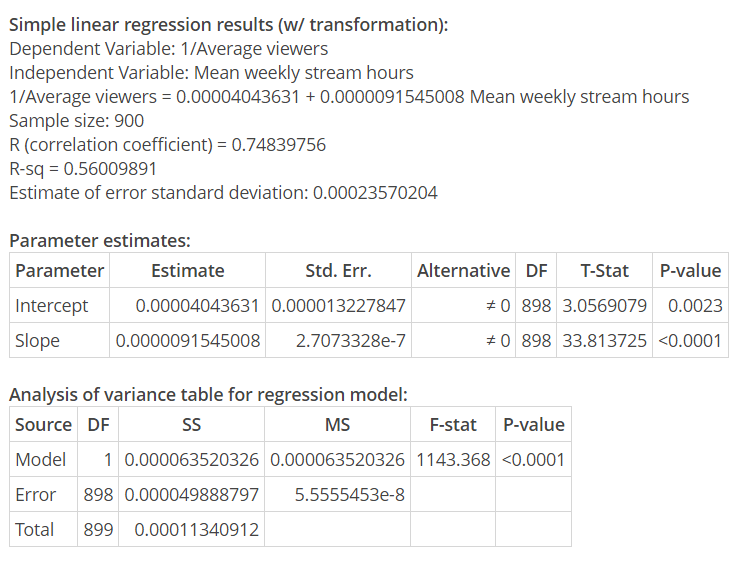
\includegraphics[width=0.8\linewidth, height=0.375\textheight]{../StatCrunch_Results/reciprocal/regression_table}
  \captionsetup{justification=centering, singlelinecheck=false, margin=2cm}
  \caption[Regression: Average Viewers Predicted by Stream Hours]{Simple linear regression model showing a moderate relationship between average viewers and mean weekly stream hours.}
  \label{table:reciprocal_regression_table}
\end{table}

R-squared is moderate, suggesting that the mean weekly stream hours can explain 56 percent of the variation in the average number of viewers. Because of the inverse transformation of the dependent variable, the signs of the intercept and mean weekly stream hours coefficient are reversed. This makes sense though, since an increase in the denominator of the equation (when the right hand side of the equation is back transform; Eq. \ref{eq:back_transformed}) will diminish the predicted number of average viewers.

\begin{equation}
Average\ viewers_{i} = \dfrac{1}{4.04e^{-5} + 9.15e^{-6} \ast Mean\ weekly\ stream\ hours_{i}} \label{eq:back_transformed}
\end{equation}

Figure \ref{fig:stream_time_reciprocal_avg_viewers} shows the relationship between the mean weekly stream hours and the inverse of average viewers. The other scatter plots show the residuals. The histogram and Q-Q plots show that the residuals are now nearly normal, although excess kurtosis is still high, making the distribution of the residuals leptokurtic (skewness = -0.57036091; excess kurtosis = 6.0727871). Removing extreme dependent variable observations would help correct for this, but it is unlikely to be helpful since inference is not being conducted. Heteroskedasticity also was not corrected, but it also is not an issue as no hypothesis testing is being conducted, nor are confidence intervals being calculated.


%%%%%%%%%%%%%%%%%%%%%%%%
% stream_time_reciprocal_avg_viewers
%%%%%%%%%%%%%%%%%%%%%%%%
\begin{figure}[!b]
  \centering
  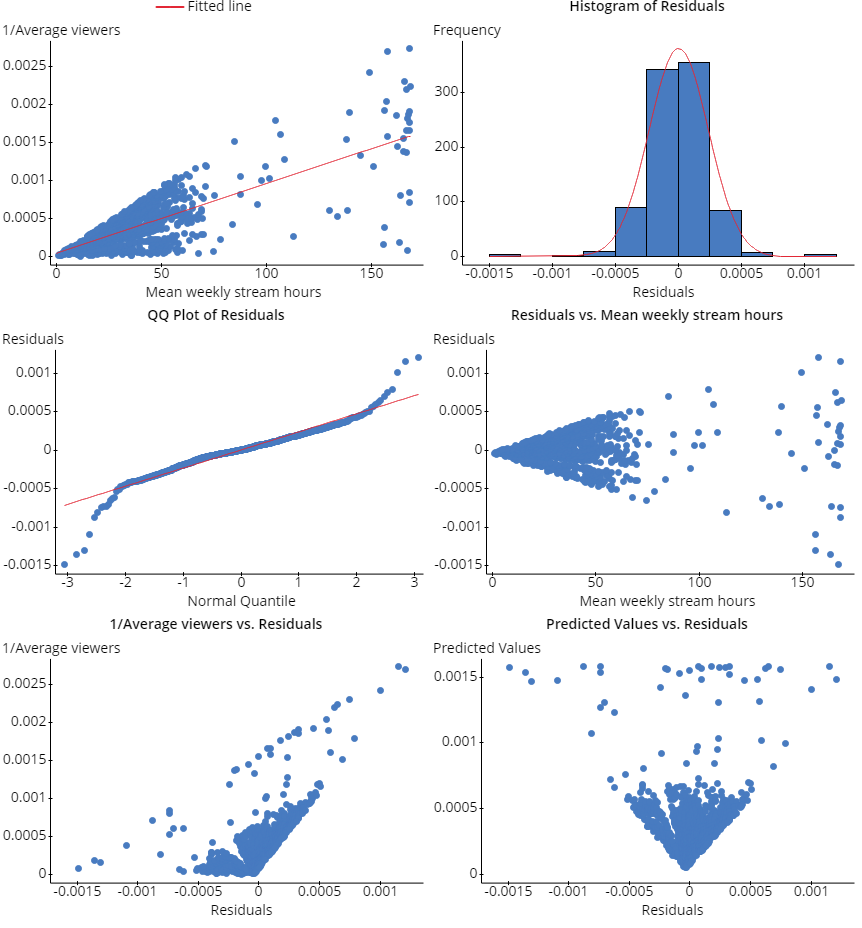
\includegraphics[width=0.8\linewidth, height=0.4\textheight]{../StatCrunch_Results/reciprocal/stream_time_reciprocal_avg_viewers}
  \captionsetup{justification=centering, singlelinecheck=false, margin=2cm}
  \caption[Residuals: Average Viewers Predicted by Stream Hours]{Residual Plots of the model. There residuals are symmetric, making the model a decent fit, nothwithstanding the non-constant variance.}
  \label{fig:stream_time_reciprocal_avg_viewers}
\end{figure}


%%%%%%%%%%%%%
% Figure: Histogram Matrix
%%%%%%%%%%%%%
\begin{figure}
  \centering
  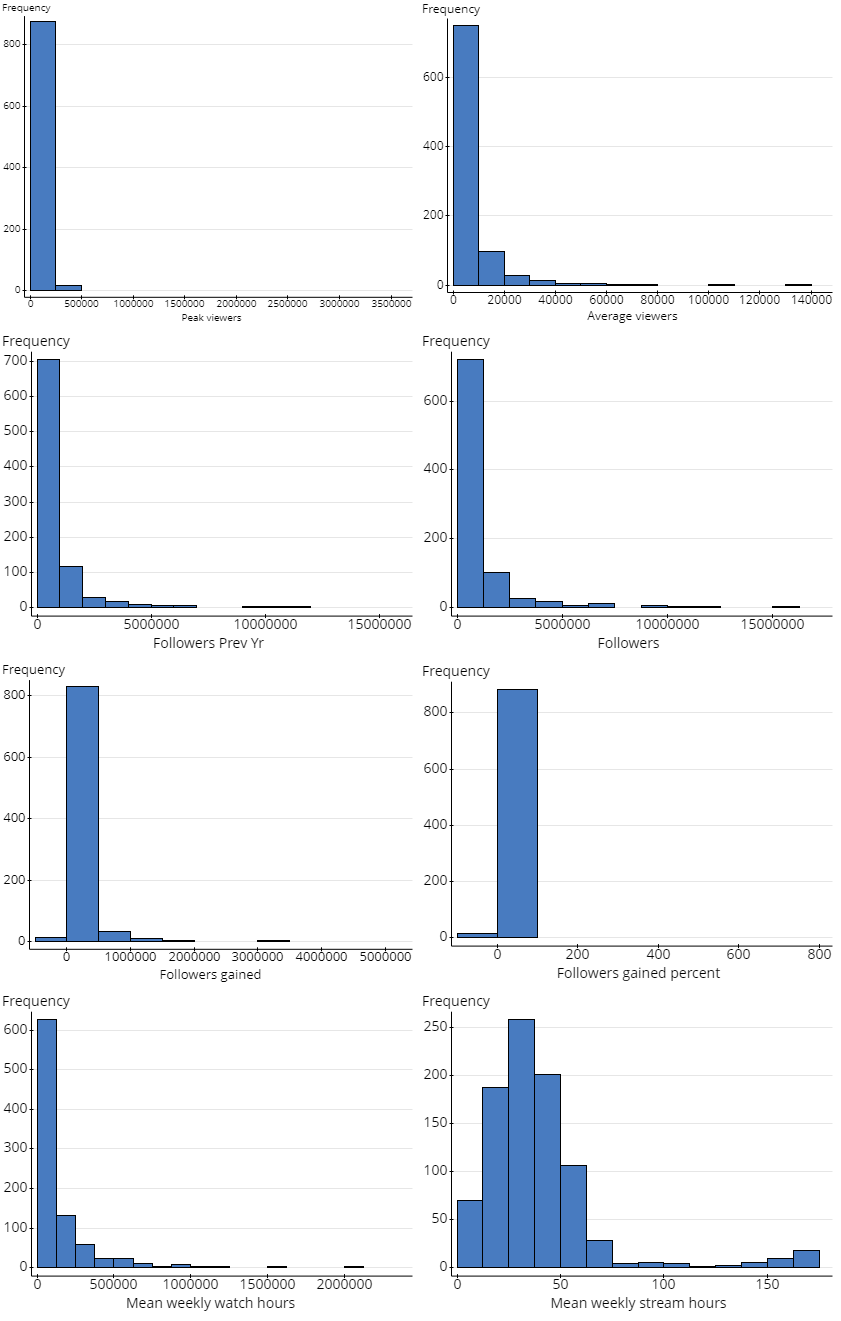
\includegraphics[width=0.8\linewidth]{../StatCrunch_Results/Histogram_Matrix.png}
  \captionsetup{justification=centering, singlelinecheck=false, margin=2cm}
  \caption[Histogram Matrix]{All distributions are heavily skewed and non-normal.}
  \label{fig:histogram_matrix}
\end{figure}

%%%%%%%%%%%%%%%%%%%
% Figure: Stream Hours Scatter Plot Matrix
%%%%%%%%%%%%%%%%%%%
\begin{figure}
  \centering
  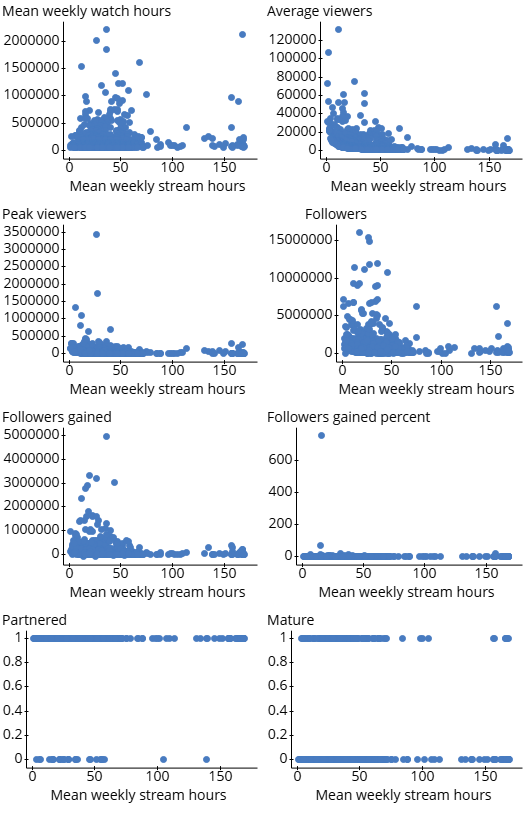
\includegraphics[width=0.8\linewidth]{../StatCrunch_Results/stream_scatter_plot_matrix.png}
  \captionsetup{justification=centering, singlelinecheck=false, margin=2cm}
  \caption[Stream Hours Scatter Plot Matrix]{Relationships between \texttt{`Mean weekly stream hours'} and other variables.}
  \label{fig:stream_scatter_matrix}
\end{figure}

%%%%%%%%%%%%%%%%%%%%%%%%%%%%%%%%%%%%%%%%%%%%
% Figure: Watch Hours Scatter Plot Matrix
%%%%%%%%%%%%%%%%%%%%%%%%%%%%%%%%%%%%%%%%%%%%
\begin{figure}
  \centering
  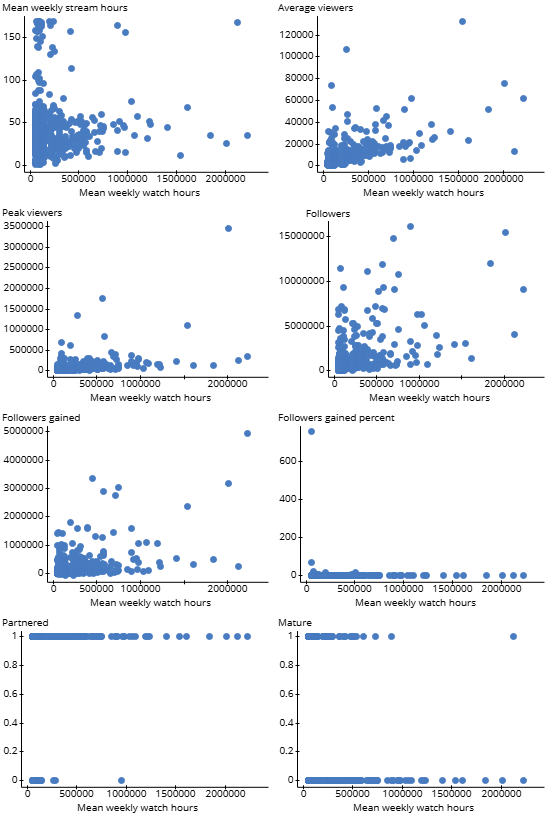
\includegraphics[width=0.8\linewidth]{../StatCrunch_Results/watch_scatter_plot_matrix.png}
  \captionsetup{justification=centering, singlelinecheck=false, margin=2cm}
  \caption[Watch Hours Scatter Plot Matrix]{Relationships between \texttt{`Mean weekly watch hours'} and other variables.}
  \label{fig:watch_scatter_matrix}
\end{figure}

%%%%%%%%%%%%%%%%%%%%%%%%
% Figure: Followers Gained Scatter Plot Matrix
%%%%%%%%%%%%%%%%%%%%%%%%
\begin{figure}
  \centering
  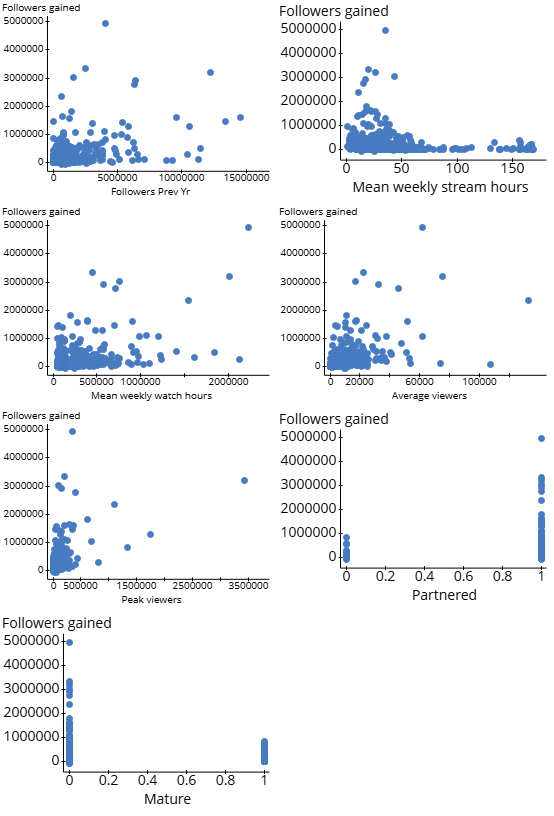
\includegraphics[width=0.8\linewidth]{../StatCrunch_Results/follow_gain_scatter_matrix}
  \captionsetup{justification=centering, singlelinecheck=false, margin=2cm}
  \caption[Followers Gained Scatter Plot Matrix]{Relationships between \texttt{`Followers gained'} and other variables.}
  \label{fig:follow_gain_scatter_matrix}
\end{figure}


% ceil(Rank(Mean weekly stream hours) / 90)

\end{document}